\chapter{Galactic Dynamics}

\section{Galactic Dynamics}

\bigskip
\subsection{Stellar distribution}\label{subsec:stardist}

The surface brightness (stellar components) of elliptical galaxy falls off smoothly with radius,
and it can be fitted by some empirical profiles:

\noi{\bf 1) S\'{e}rsic profile}

\begin{equation}\label{eq:Sersic}
    I(r) = I_{e}\,\exp{ \left\{ -\nu_{n} \left[ \left( \frac{r}{r_{e}}\right)^{1/n} - 1 \right] \right\}},
\end{equation}
where, $r_{e}$ is effective radius, the radius of the isophote containing half of the total luminosity.

\medskip
\noi{\bf 2) De Vaucouleurs profile} 

When $n=4,\,\nu_{4}=7.66925$, the S\'{e}rsic profile [eq.~(\ref{eq:Sersic})] becomes de Vaucouleurs profile,
\begin{equation}
    I(r) = I_{e}\,\exp{ \left\{ -\nu_{4} \left[ \left( \frac{r}{r_{e}}\right)^{1/4} - 1 \right] \right\}}.
\end{equation}


\medskip
\noi{\bf 3) King profile}

King profile was developed from the singular isothermal sphere model, at which the distribution function 
follows the balance between the gravitational potential and velocity dispersion (analogue to the hydrostatic 
equilibrium sphere with adiabatic index of $\gamma=1$).
\begin{equation}
    I(r) = K\,\left\{ \left[ 1 + \left( \frac{r}{r_{c}} \right)^{2} \right]^{-1/2} 
            - \left[ 1+ \left( \frac{r_{t}}{r} \right)^{2} \right]^{-1/2} \right\}^{2},
\end{equation}
where $r_{c}$ is the core radius $\left[ \frac{I(r=0)}{I(r=r_{c})}=2 \right]$, $r_{t}$ is the tidal radius where 
is considered as outermost limit of the system by observers, and $K$ is the scale factor.

This profile gives a very good representation of star counts in tidally-limited globular clusters and low-density
spheroidal galaxies.

\medskip
\noi{\bf 4) Exponential profile}

Disks of spiral galaxies are known to show profiles described well by the exponential law:
\begin{equation}
    I(r) = I_{0}\,\exp{\left( -\frac{r}{h} \right)},
\end{equation}
where $h$ is the exponential scale length.

\bigskip
\subsection{Dark matter profile: Two-power density models \cite{Binney:87}}

Numerical simulations of the clustering of dsrk matter particles suggest that the mass density with dark halo 
has a similar structure. Mostly, the two-power density models has been applied:
\begin{equation}\label{eq:twoden_dm}
    \rho(r) = \frac{\rho_{0}}{(r/a)^{\alpha}(1+r/a)^{\beta-\alpha}}.
\end{equation}
According to the sets of $(\alpha,\beta)$, the model can be classified with Jaffe, Hernquist, and NFW profiles. 
The mass interior to radidus $r$ is
\begin{equation}\label{eq:twoden_M}
    M(r) = 4\pi\rho_{0}\,a^{3} \int^{r/a}_{0} ds\,\frac{s^{2-\alpha}}{(1+s)^{\beta-\alpha}}.
\end{equation}

\medskip
\noi{\bf 1) Jaffe profile}

$\alpha=2$ and $\beta=4$ in eq.~(\ref{eq:twoden_dm}).
Therefore, from eq.~(\ref{eq:twoden_M}), the mass profile becomes
\begin{equation}
    M(r) = 4\pi\rho_{0}\,a^{3} \frac{r/a}{1+r/a},
\end{equation}
and the potential becomes
\begin{eqnarray}
    \Phi(r) &=& -G\int^{\infty}_{r} dr\,\frac{M(r)}{r^{2}} \nonumnext
            &=& -4\pi\rho_{0}\,a^{2}\, \ln{(1+a/r)}.
\end{eqnarray}

\noi{\bf 2) Hernquist profile}

$\alpha=1$ and $\beta=4$ in eq.~(\ref{eq:twoden_dm}).
Therefore, from eq.~(\ref{eq:twoden_M}), the mass profile becomes
\begin{equation}
    M(r) = 4\pi\rho_{0}\,a^{3} \frac{(r/a)^{2}}{2(1+r/a)^{2}},
\end{equation}
and the potential becomes
\begin{eqnarray}
    \Phi(r) &=& -G\int^{\infty}_{r} dr\,\frac{M(r)}{r^{2}} \nonumnext
            &=& -4\pi\rho_{0}\,a^{2}\, \frac{1}{2(1+r/a)}.
\end{eqnarray}


\noi{\bf 3) NFW profile}

NFW profile is named from Navarro, Frenk, \& White (1995).
$\alpha=1$ and $\beta=3$ in eq.~(\ref{eq:twoden_dm}).
Therefore, from eq.~(\ref{eq:twoden_M}), the mass profile becomes
\begin{equation}
    M(r) = 4\pi\rho_{0}\,a^{3} \left[ \ln{(1+r/a)} - \frac{r/a}{1+r/a} \right],
\end{equation}
and the potential becomes
\begin{eqnarray}
    \Phi(r) &=& -G\int^{\infty}_{r} dr\,\frac{M(r)}{r^{2}} \nonumnext
            &=& -4\pi\rho_{0}\,a^{2}\, \frac{\ln{(1+r/a)}}{r/a}.
\end{eqnarray}


\bigskip
\subsection{Fundamental Plane}
Fundamental plane is an empirical relationship of observed elliptical galaxies between the
effective radius $r_{e}$ (see \S\ref{subsec:stardist}), average surface brightness $I$ (or
Luminosity $L_{\rm B}$), and central velocity dispersion $\sigma_{0}$ (Fig.~\ref{fig:fundp}).
\begin{equation}
    \log{r_{e}} = A\,\log{\sigma_{0}} + B\,\log{L_{\rm B}} + C.
\end{equation}

\begin{figure}[!htbp]
    \centering
    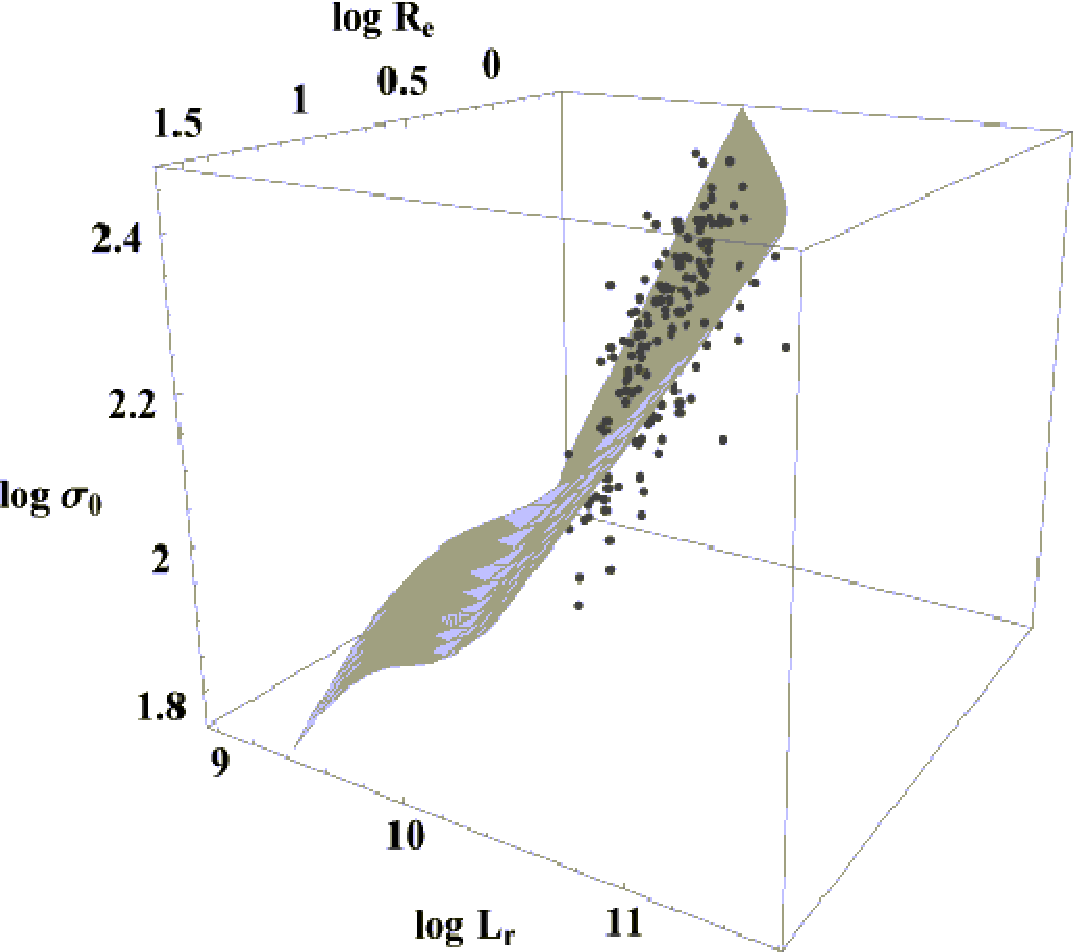
\includegraphics[width=0.7\textwidth]{Galactic/fundamentalplane}
    \caption{3 dimensional space ($r_{e},\,\sigma_{0},\,L$) of Fundamental Plane}
    \label{fig:fundp}
\end{figure}

\bigskip
\subsection{Faber-Jackson relation}
This relation is an empirical power-law relation between the luminosity $L$ and the central 
stellar velocity dispersion $\sigma_{0}$ of elliptical galaxies. 

The theoretical derivation requires some assumptions:

The gravitational potential for uniform sphere (constant density; see \S\ref{subsec:potunisp}) is 
\begin{equation}
    U = -\frac{3}{5} \frac{G\,M}{R}.
\end{equation}
And the kinetic energy is 
\begin{equation}
    K = \frac{3}{2} M\,\sigma_{0}^{2},
\end{equation}
where $\sigma_{0}$ is 1-dimensional velocity dispersion ($3\sigma_{0}^{2} = V^{2}$ where $V$
is total velocity dispersion). From the virial therom ($2K+U=0$), it follows
\begin{equation}
    \sigma^{2}=\frac{1}{5}\frac{G\,M}{R}.
\end{equation}
Assuming the constant mass to light ratio $\Upsilon=M/L$, then 
\begin{equation}
    R = \frac{1}{5}\frac{\Upsilon L\,G}{R}.
\end{equation}
If we assume that the surface brightness $I=L/(4\pi R^{2})$ is constant (highly unlikely),
then
\begin{equation}
    L = \frac{25\,\sigma^{4}}{4\pi\,G^{2}\,I\,\Upsilon^{2}} \propto \sigma^{4}.
\end{equation}
Since the assumptions during the derivation are poor, the empirical power varies between 3 (less massive galaxies) 
and 15 (more massive galaxies).

\bigskip
\subsection{Tully-Fisher relation}
The rotation rate of spiral galaxies in the flat part of the circular-speed curve is
related to their luminosity.

\bigskip
\subsection{Nearly circular orbits: Epicycle frequency}
In disk galaxies, many stars are on nearly circular orbits. We define
\begin{equation}
   x \equiv r - r_{g},
\end{equation}
where $r_{g}$ is the guiding center radius for an orbit.
The effective potential is 
\begin{equation}
   \Phi_{\rm eff} = \Phi + \frac{l^{2}}{2\,r^{2}},
\end{equation}
where $l$ is a specific angular momentum $l = r\,v_{\phi}$, and $v_{\phi}$ is rotation velocity.
Expanding $\Phi_{\rm eff}$ in a Taylor series results in
\begin{equation}\label{eq:PhieTyl}
    \Phi_{\rm eff} (r) = \Phi_{\rm eff}(r_{g}) + \left. \frac{\partial \Phi_{\rm eff}}{\partial r} \right|_{r=r_{g}} x
                    + \frac{1}{2} \left. \frac{\partial^{2} \Phi_{\rm eff}}{\partial r^{2}} \right|_{r=r_{g}} x^{2} + O(x^{2}).
\end{equation}
The first order term (second term in RHS) vanishes because $\Phi_{\rm eff}$ is assumed to be symmetic about $r=r_{g}$.
So the eq.~(\ref{eq:PhieTyl}) can be approximated to 
\begin{equation}
    \Phi_{\rm eff} (r) \simeq \Phi_{\rm eff}(r_{g}) 
                    + \frac{1}{2} \left. \frac{\partial^{2} \Phi_{\rm eff}}{\partial r^{2}} \right|_{r=r_{g}} x^{2} 
\end{equation}
The equation of motion is
\begin{eqnarray}
    \ddot{x} = -\frac{\Phi_{\rm eff}}{x} &=& - \left. \frac{\partial^{2} \Phi_{\rm eff}}{\partial r^{2}} \right|_{r=r_{g}} x \\
             &=& -\kappa^{2}\,x,
\end{eqnarray}
where $\kappa$ is called \emph{epicycle frequency}.
\begin{equation}\label{eq:epi1}
    \kappa^{2}(r_{g}) = \left. \frac{\partial^{2} \Phi_{\rm eff}}{\partial r^{2}} \right|_{r=r_{g}}
             = \left. \frac{\partial^{2} \Phi}{\partial r^{2}} \right|_{r=r_{g}} + \frac{3\,l^{2}}{r_{g}^{4}}.
\end{equation}
Since the circular frequency is related with the gravitational force,
\begin{equation}
    \frac{\partial \Phi}{\partial r} = r\, \Omega^{2},
\end{equation}
where $\Omega = l/r^{2}$ is an angular frequency of the circular orbit. Plugging into eq.~(\ref{eq:epi1}) gives
\begin{eqnarray}\label{eq:epi2}
    \kappa^{2}(r_{g}) &=& \left( r \frac{d\,\Omega^{2}}{d\,r} + 4\,\Omega^{2} \right)_{r=r_{g}} \\
                      &=& \left[ \frac{1}{r^{3}} \frac{d}{d\,r} \left( r^{4}\,\Omega^{2} \right) \right]_{r=r_{g}}.
\end{eqnarray}
If we assumes that the angular frequency has a power-law relationship with the radius ($\Omega \sim r^{q}$),
the eq.~(\ref{eq:epi2}) can be expressed as
\begin{equation}
    \kappa^{2} = (4 + 2q)\,r^{2q} = (4 + 2q)\,\Omega^{2}.
\end{equation}
Note the several examples of the epicycle frequency:
\begin{empheq}[left=\empheqlbrace]{align}
    {\rm Rigid~ rotation} &:      \Omega \sim R^{0} \rightarrow \kappa^{2} = 4\Omega^{2} \\
    {\rm Keplerian~ rotation} &:  \Omega \sim R^{-3/2} \rightarrow \kappa^{2} = \Omega^{2} \\
    {\rm Flat~ rotation} &:       \Omega \sim R^{-1} \rightarrow \kappa^{2} = 2\Omega^{2} 
\end{empheq}
In the rigid and Keplerian rotations, the epicycle motion is closed, but in the flat rotation 
it is not closed.

\bigskip
\subsection{Luminosity function: Schechter law}
The luminosity function $\phi(L)$ describes the relative numbers of galaxies of different luminosities,
and is defined so that $\phi(L)\,dL$ is the number of galaxies in the luminosity interal $L \rightarrow L+dL$
in a representative unit volume of the universe. The analytic approximation is know as Schechter law:
\begin{equation}
    \phi(L)\,dL = \phi_{\star} \left( \frac{L}{L_{\star}} \right)^{\alpha} \exp{\left(-\frac{L}{L_{\star}}\right)}\frac{dL}{L},
\end{equation}
where $\phi_{\star} \simeq 4.9\times10^{-3}\,{\rm Mpc^{-3}},\,\alpha=-1.1,\,{\rm and}\, L_{\star}\simeq 2.9\times10^{10}\,L_{\odot}$
in the $R$ band.

\bigskip
\subsection{Star Formation Rate: Kennicutt-Schmidt Law}
Kennicutt-Schmidt law is the empirical relationship between the global star formation in a galaxy 
and $\Sigma_{\rm gas,disk}$ the gas surface density averaged over the ``optical disk'' of the galaxy, finding
that the star formation rate per unit area $\Sigma_{\rm SFR,disk}$ varies approximately as
\begin{eqnarray}
    \Sigma_{\rm SFR,disk} &=& (2.5\pm0.7)\times 10^{-4} \left( \frac{\Sigma_{\rm gas,disk}}{M_{\odot}{\rm pc^{-2}}} \right)^{1.4\pm 0.15}\,M_{\odot}\,{\rm kpc^{-2}{yr^{-1}}} \\
                          &\propto& \Sigma_{\rm gas,disk}^{1.4}.
\end{eqnarray}

\bigskip
\subsection{Initial Mass Function (IMF): Salpeter or Kroupa}
According to single burst stellar population synthesis models, most of the stellar mass is lost 
at early times, before an age of $\sim 2$ Gyr: 25\% and 36\% of the total initial mass are lost
for the Salpeter and Kroupa IMF, respectively. The approxmiated model\cite{Kim:13} is:
\begin{equation}
    \dot{M}_{\star}(t) = 10^{-12}\,A\times \left( \frac{M_{\star}}{M_{\odot}} \right) t_{12}^{-1.3}~~~M_{\odot}{\rm yr^{-1}},
\end{equation}
where $M_{\star}$ is the galactic stellar mass at an age of 12 Gyr, $t_{12}$ is the age in units of 12 Gyrs,
and $A=2.0~{\rm or}~3.3$ for a Salpeter or Kroupa IMF.
